	\large \bf{\textsc{\section{Lab 3}}
	\begin{problem}
		Choose a diode type 1N4001 and build the following circuit.\\	
		R=100 \(\Omega\) (potentiometer) \\ 
		D is 1N4001 \\
		E=2v (max current I$_{max}$=350mA)
		\newline\newline
		1. Measure the diode and resistor voltage and current when changing the resistor R and fill the table
		\newline
		2. Plot the I-V characteristics  of the diode as well as the resistor. Are all measurements on one line? Are the components linear? Compare the diode i-v plot with the datasheet.
		
		\begin{figure}[h!]
			\centering
			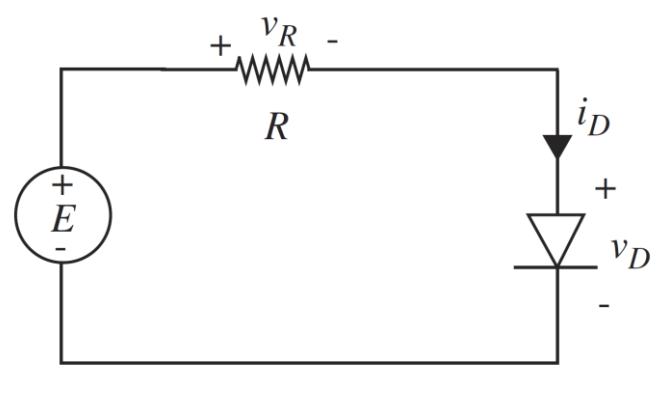
\includegraphics[width=0.5\textwidth]{images/circuit1.png}
		\end{figure}
	\end{problem}
	
	\begin{solution}
		1.
		\begin{table}[h]
			\begin{tabular}{| l | l | l | l | l | l | l | l | l | l | l | l |}
				\hline
				Try          & 1 & 2 & 3 & 4 & 5 & 6 & 7 & 8 & 9 & 10 & 11 \\ \hline
				R (\(\Omega\))   &   &   &   &   &   &   &   &   &   &    &    \\ \hline
				V$_{D}$ (V)  &   &   &   &   &   &   &   &   &   &    &    \\ \hline
				V$_{R}$ (V)  &   &   &   &   &   &   &   &   &   &    &    \\ \hline
				i$_{D}$ (mA) & 20 & 30 & 50 & 80 & 120 & 160 & 200 & 240 & 280 & 320 & 350 \\ \hline
			\end{tabular}
		\end{table}
		\newline
		2.
	\end{solution}
	
	\begin{problem}
		In this exercise, we would like to build a full wave rectifier using a diode bridge.
		\newline
		1. Construct the following circuit using:\\
		R\(_{L}\)=10K\(\Omega\)\\
		D is 1N4001\\
		V\(_{i}\)=20sin(100\(\pi\)t)\\
		\newline
		2. Measure the input voltage and current using a multimeter.
		\newline
		3. Measure the output voltage on R\(_{L}\) using a multimeter and an oscilloscope.
		\newline
		4. Compare the measurements with your calculations
		\newline
		5. (Optional) Use a 470\(\mu\)F capacitor in parallel with R\(_{L}\) and measure the output voltage.
		\begin{figure}[h!]
			\centering
			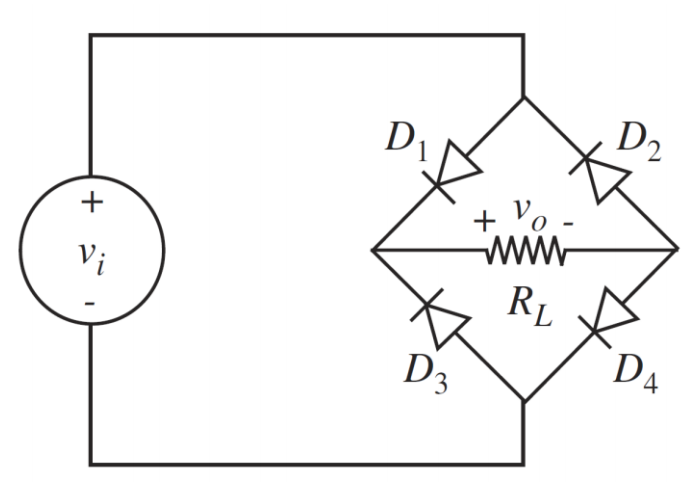
\includegraphics[width=0.5\textwidth]{images/circuit2.png}
		\end{figure}
	\end{problem}
	
	\begin{solution}
		1.
		\newline
		2.
		\newline
		3.
		\newline
		4.
		\newline
		5.
	\end{solution}
	
	\begin{problem}
		Using an OpAmp TL082, construct an inverting amplifier of gain 2.
		\newline
		V\(_{i}\)=1.5v\\
		V\(_{CC}\)=12v\\
		Output current should not exceed 10mA
		\newline
		1. Measure the output voltage and compare with your expectations.
		\newline
		2. Use V\(_{i}\)=2sin(100\(\mu\)t) and measure the output voltage using an oscilloscope.
		\begin{figure}[h!]
			\centering
			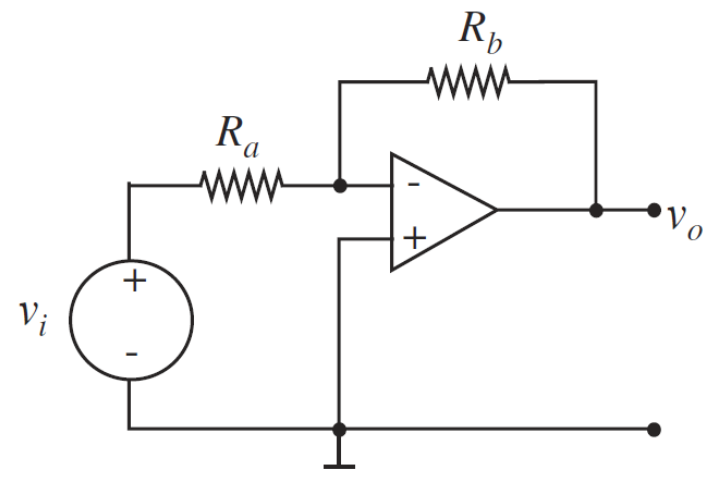
\includegraphics[width=0.5\textwidth]{images/circuit3.png}
		\end{figure}
	\end{problem}
	
	\begin{solution}
		1.
		\newline
		2.
	\end{solution}